\documentclass[12pt]{article}
\usepackage{fullpage}
\usepackage{graphicx}
\begin{document}
\title{Data-Vis Assignment 2}
\author{Jack Cassidy \\ Student Number: 1432 0816}
\date{\today}
\maketitle
\section{Related Readings}
From a data visualization perspective, there are two categories of data that we are concerned with: ordinal and nominal. Ordinal data, as the name suggests, implies that there is an inherit order/rank to the data items, but the magnitude of the \textit{difference} between values cannot be quantified. Conversely, nominal data has no ordering. An example of ordinal data would be satisfaction rating on a survey, such as "Very Unsatisfied", "Unsatisfied", "Neither Satisfied nor Unsatisfied", "Satisfied", "Very Satisfied". The data does not necessarily have to be numeric, but there is an order to these values. An example of nominal data would be gender, hair color or marital status.

\subsection{What are the main ways of encoding data in visualization?}
"Marks are basic geometric elements that depict items or links, and channels control their appearance." \cite{munzner} The fundamental marks used are points (0D), lines (1D) and areas (2D). We can move to 3D and express marks as surfaces, but they are generally reserved for niche applications such as scientific or mathematical visualizations. Channels are used to encode data attributes into marks so that they can be expressed visually to the viewer. The main channels used are position, shape, size, brightness, colour, orientation, texture and motion. For example, a scatter plot of audio noise levels across a city may visualize the data as a series of \textit{point} marks with a \textit{size} channel to convey the noise level magnitude. \\

There are 5 characteristics used to qualify the use of a channel. They are as follows.
\begin{itemize}
	\item Selective: Can one mark be visually distinguished from another.
	\item Associative: Can marks be grouped based on the channel properties.
	\item Quantitative: Can the magnitude of the difference between two marks be quantified.
	\item Ordinal: Can marks be ordered/ranked based on the channel properties.
	\item Range: How many unique marks can be produced.
\end{itemize}

As an example, the colour channel is selective, associative and has a limited range. It is not quantitative or ordinal. There are two principles that govern the selection of any visual channel. The relative performance of each channel when applied to a unique dataset can be quantified using the metrics of accuracy, discriminability, separability, popout and grouping. \\

Accuracy being the most obvious metric can actually give a numeric, mathematically derived figure to rank a channel based on perceived sensation by the viewer. It is defined as
\begin{center}
	$\psi(I) = I^a$
\end{center}
Where $\psi$ is the perceived intensity of the channel, $I$ is the magnitude of the stimulus, $a$ is a constant factor dependant on the channel. Accuracy gives the perceived effectiveness of the stimulus with respect to it's intended effectiveness. \\

Discriminability describes the level of perceptible difference between marks encoded with the same channel. The shape channel can be used with a high level of discriminability, however line size may not be as performant in this metric as one might assume. It works for a relatively small number of steps and is dependant on the maximum width of the line and step size. \\

Separability defines the relationship between combinations of channels, more specifically it describes how differentiable they are when used together. Lack of separability is not inherently a negative attribute, it all depends on the underlying dataset. \\

Popout defines how much a distinct data item stands out from the remaining data. Popout is highly dependant on the combination of channels used and in general starts to decay as more channels are used. Size and colour are a combination with good popout, they can be leveraged to point out outliers easily as their combined range is quite high. \\

Grouping arises from creating link marks, such as edges of a graph or container outlines around other marks, to give the perception of similar or related data.

The \textit{expressiveness principle} states that the channel must express all of, and only the information in for dataset attributes, that is to say that no unwarranted or noise data leaks into the visual encoding. A simple example of a breach of this principle would be a portrayal of ordering of data in the visualization of a dataset with no ordering. The \textit{effectiveness principle} states that the notability or relative importance of the channel should match that of the underlying attribute.
\subsection{What are some reccuring types of datasets in visualization?}
To understand datasets, we must first understand the five most basic data types. These types are atomic, and combine to form the fundamental datasets that we will discuss.
\begin{itemize}
	\item Attribute: A measurable quality, feature, characteristic or inherent part of something.
	\item Item: An atomic entity, that is usually described by a set of attributes.
	\item Link: Represents a relationship between items. Can often be thought of as an edge between nodes in a graph.
	\item Position: Spatial information.
	\item Grid: Discrete sampling of continuous data. Not necessarily a set of uniform cells bounded by horizontal and vertical lines.
\end{itemize}

The four basic dataset types are tables, networks/graphs, fields and geometry/spatial. The simplest of these to understand is the table, a collection of items representing rows, and attributes representing columns. A cell is an indivisible object of data specified by a row, column pair. \\

A network/graph is generally used to represent some kind of relationship between data items, often referred to as nodes in this context. Relationships are represented with link marks. An example of a network database might be a visualization of Facebook profiles, where a node represents a person and a link a friendship between two people. A tree is a special case of a graph, where there is a definite hierarchy between nodes and there are no cycles. \\

Fields are similar to tables in that data objects are conveyed in cells indexed by row, column pairs. However the cells in a field contain data that has been sampled from a continuous domain, such as a human body temperature scan or a plot of a sound wave. \\

Geometry/spatial datasets are different to the previously mentioned types as they do not necessarily contain data attributes. They are used to portray spacial information with exact geometries, such as lines and curves, surfaces and volumes, geographical information etc. They are used in visual representations that require spatial understanding.
\subsection{What are the reccuring types of tasks in visualization?}
The visualization pipeline is often made up of a set of fundamental tasks that must be carried out on the dataset, in tandem with exploring the type of data that is present. It is not enough to simply choose the visualization based on the data types alone.
\begin{itemize}
    \item Analyse: Analysis of the dataset can be separated into two high level tasks: consume and produce. Consuming data involves looking at the data collectively and forming a conclusion or hypothesis that is worth visualizing. Producing data is the process of generating new data from what was previously there. This process can include a combination of annotating data usually graphically in order to better explain what the data represents, recording dynamic data such as video data as persistent artefacts, and derive new features from underlying data which might imporve the understanding or readability of the visualization.
	\item Search: As the name suggests, search involves finding a target set of data from the dataset. This task varies in complexity with the amount of knowledge the user has of the target and it's location. Search has 3 types: 
	\begin{itemize}
		\item Lookup: The location is known
		\item Locate: The location is unknown
		\item Browse: A characteristic of the data is known, which might aid in locating it
	\end{itemize}
    \item Query: Queries follow on from a search result. They return requested characteristic/attributes of the resulting target, as not all of the information is always needed. Queries can combine the entire search results to compare and contrast results in a summary, do the same with just a selection of some features of the result, or they can identify just a single target. 
\end{itemize}

\section{Analyzing Visualizations}
\subsection{American Workday, By Occupation}
This visualization captures the location of American workers in different occupations at different times of the day \cite{workday}. Note that the visualization is animated to show behaviour throughout the day, below is a still frame captured at an interesting time.

\begin{figure}[h]
	\centering
	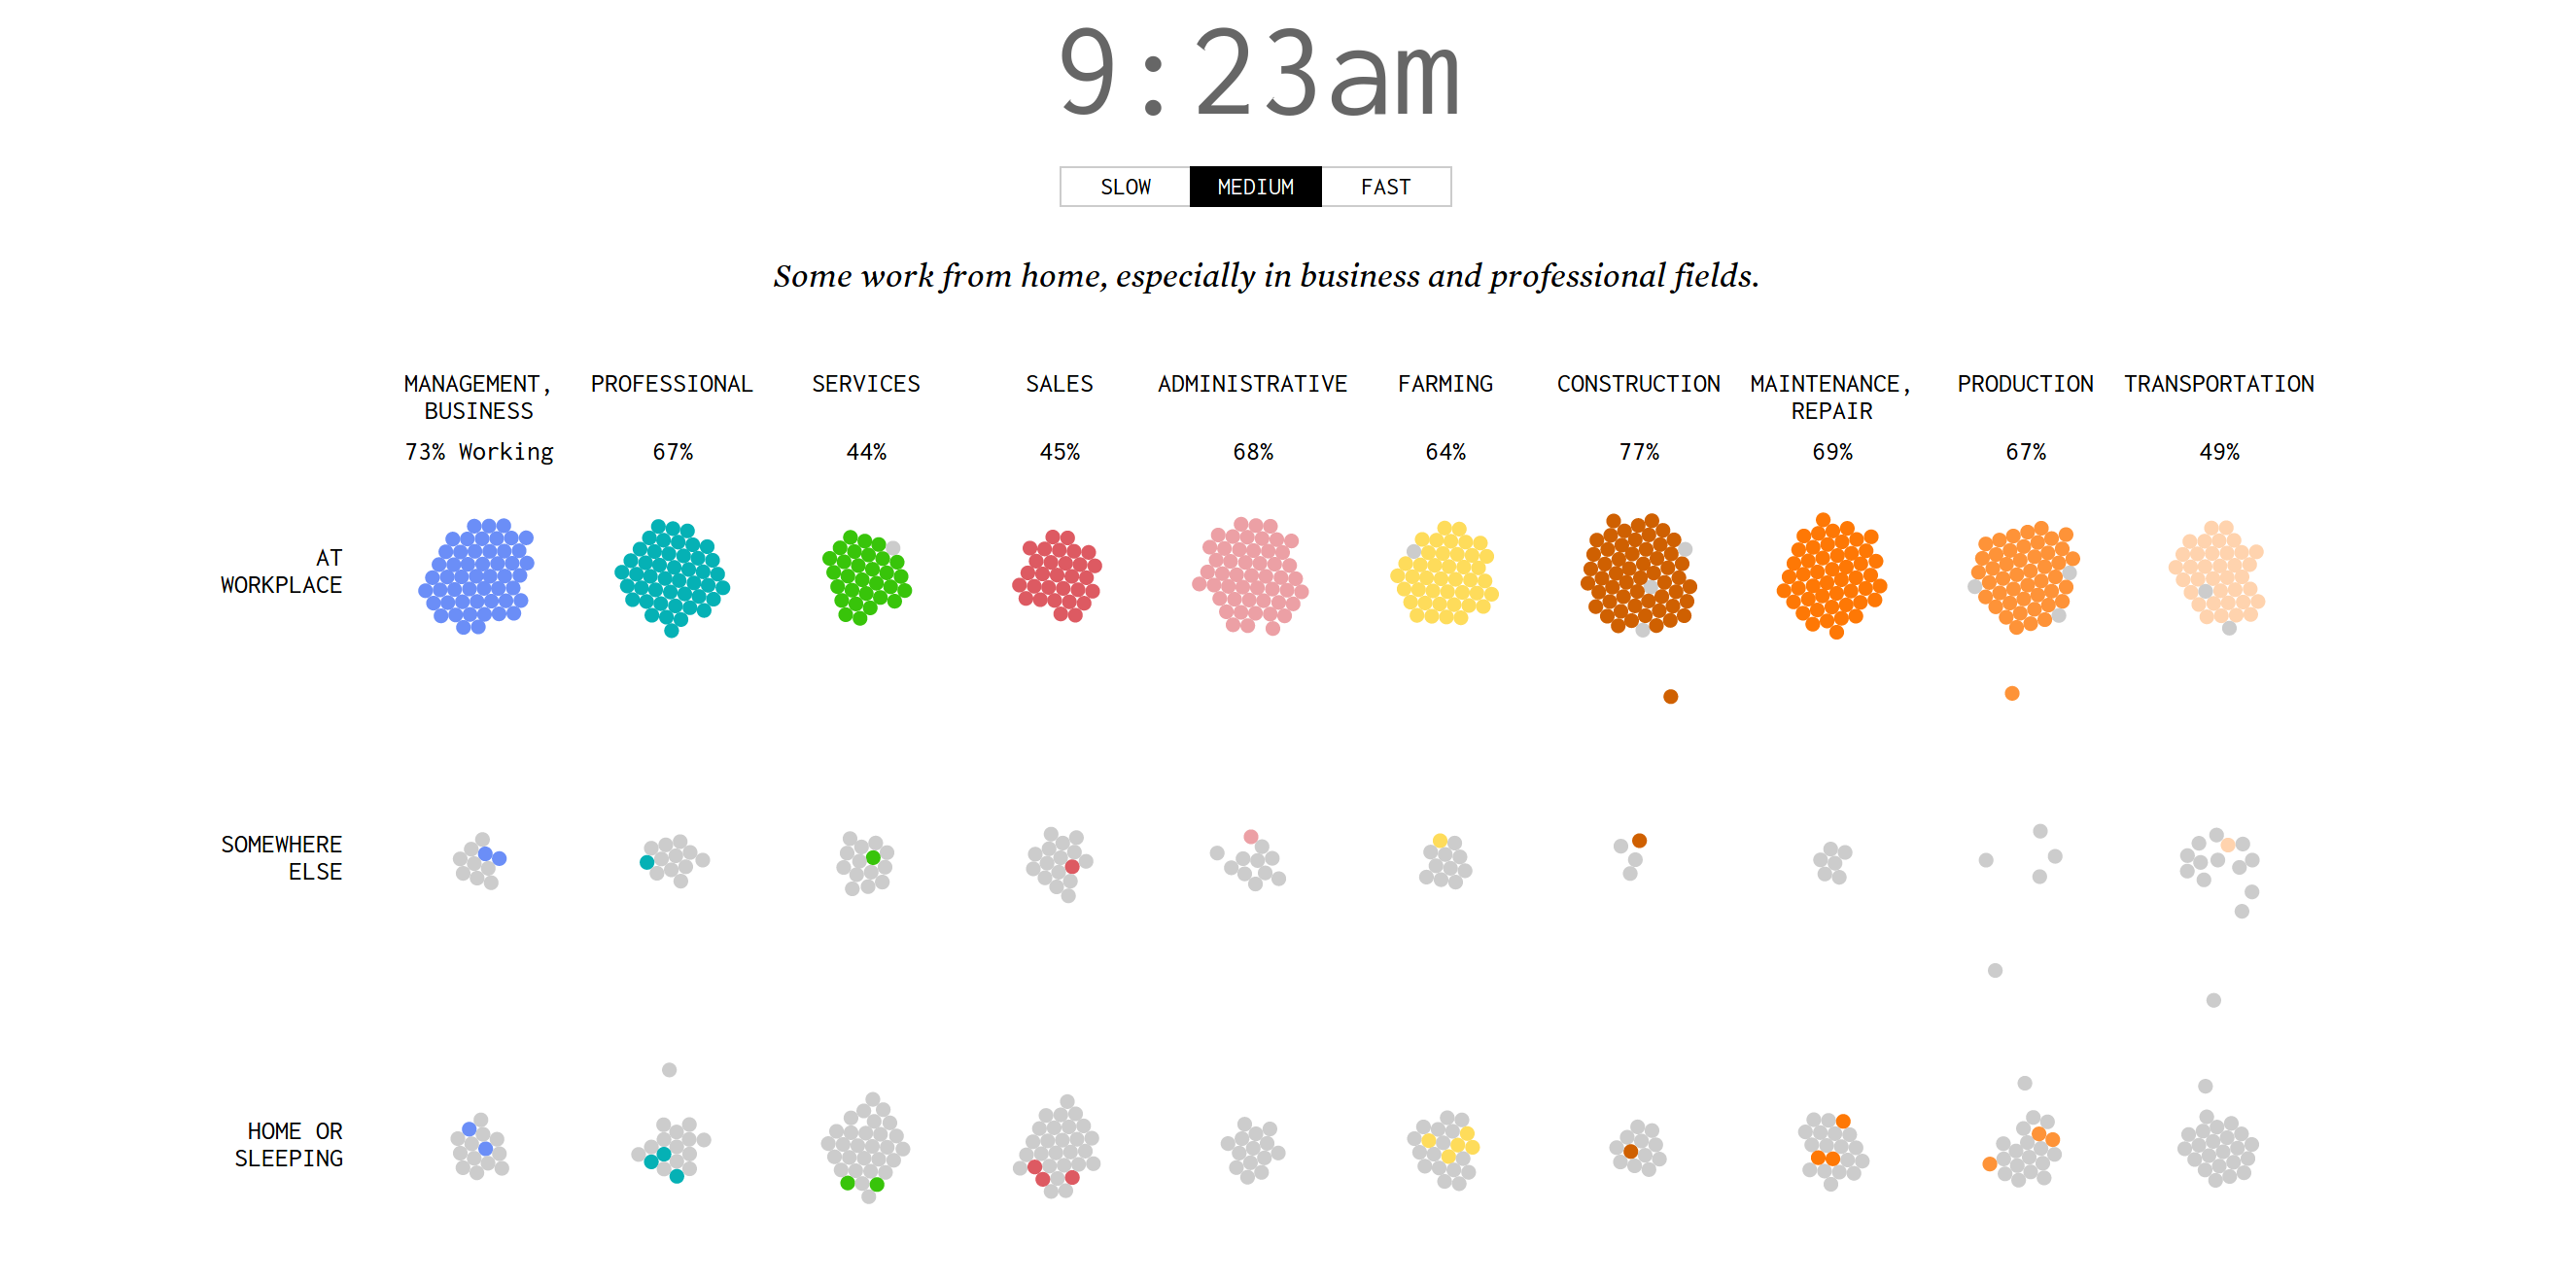
\includegraphics[scale=0.17]{workday}
\end{figure}

The dataset for this visualization requires purchasing it from \texttt{www.atusdata.org/atus}, hence we cannot directly see the types of the underlying data. The dataset was compiled by the American Time Use Survey, who conduct censuses yearly to assemble this type of data. The locations are categorised into 'At Workplace,' 'Somewhere Else,' and 'Home or Sleeping.' The main visual encoding channels at play are position, size, motion and color. A certain percentage of the work population for a given occupation are encoded in circular marks and color is used to differentiate the different occupations. The position of each mark is categorised into the three locations outlined above. Motion is used in combinations with a time display to highlight the transitions of workers between the locations at different times of the day. As the colored marks cluster together, we get a rough proportion comparison between all of the occupations in all of the locations. This channel becomes quite noisy in the midday as the majority of workers are 'At Workplace' and no discernible difference can be made between the occupations. \paragraph{}

In my opinion, when viewing this dataset in its animated form, it is a very elegant visualization that makes good use of the motion encoding channel, one that is perhaps not used as frequently. Overrall we can draw interesting information from this visualization, such as how late workers in the different occupations work, how early they start and how long they work on average. One criticism I would have is that the occupation category 'professional' is quite broad and might be hard to discern from 'management, business.'

\subsection{Heat Map of 1,058,383 Basketball Shots from NCAA Games}
This is an interesting visualization showing the number of shots scored from various positions on the court over a sample of 1,058,383 shots \cite{basketball}. Credit goes to user minimaxir from \texttt{www.reddit.com/r/dataisbeautiful}. The data used was taken from the Sportsradar tabular dataset, hosted on the Google BigQuery cloud platform (\texttt{https://console.cloud.google.com/launcher/details/ncaa-bb-public/ncaa-basketball}). This is a very large dataset, with various statistics from NCAA (National Collegiate Athletic Association) basketball games from as far back as 1894.

\begin{figure}[h]
	\centering
	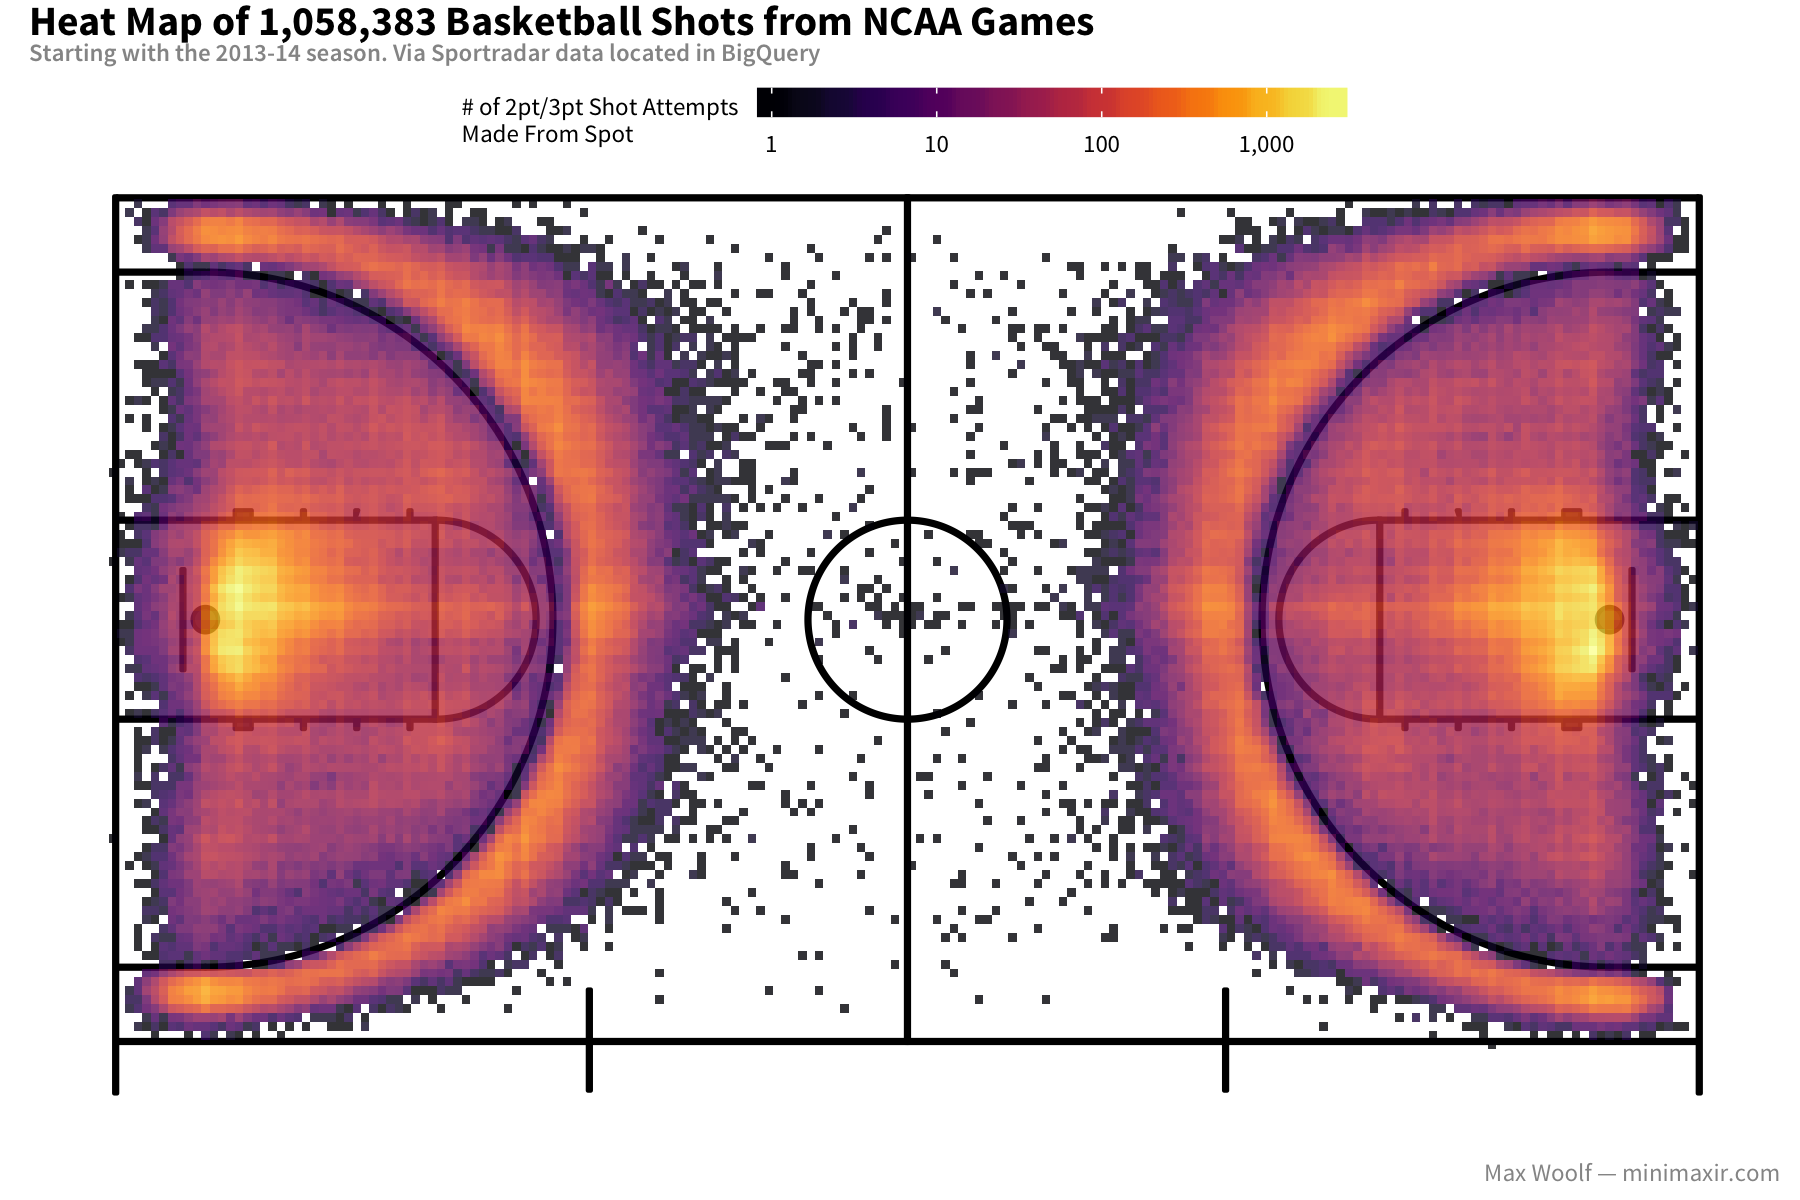
\includegraphics[scale=0.25]{basketball}
\end{figure}

The location data is given as an integer number of inches from the left baseline and an integer number of inches from the top baseline in an x,y co-ordinate type manner. For each position there is an event type, which may or not be a shot, and an indicator of whether the shot was on target. This becomes a simple task of querying all shot events and their successes and grouping them based on location. I would image that there is some discretization of the location points to form the heat map grid, such as to cluster based on ranges of location rather than on exact points. Once the points are grouped based on location, a color scale can be applied to each heat map grid point based on min-max scaling of the number of shots taken. Hence, a heat value has been derived from location points and event data to rank each position in the grid.

\begin{center}
	$heat = \frac{shots_i - min shots}{max shots - min shots}$
\end{center}

In my opinion, this visualization does a good job of conveying the information that it is intended to. The choice of colors for the heat map scale ensures that it is easy to distinguish 'hot' areas from 'cold' as they are quite contrasting. It gives an analyst a lot of information in a quite simple representation, such as where the best place to take a 3-point shot is, that shot data is alost symetrical in both x and y except for 'dunking' shots where the left side of the basket seems to be slightly favoured.

\bibliography{sample}
\bibliographystyle{plain}
\end{document}